\chapter{Implementace}\label{chapter:implementace}

V této kapitole popíšeme postup implementace aplikace.
Nejdříve představíme technologie a knihovny, které jsme k vývoji použili.
Dále uvedeme uživatelskou dokumentaci, kde popíšeme fungování a způsob použití aplikace z pohledu uživatele.
Následně se v technické dokumentaci budeme věnovat ze širšího pohledu zdrojovému kódu, konkrétně jednotlivým modulům a komponentám a jejich účelu.
Posléze se budeme věnovat tomu, jak připravit své vývojové prostředí k vývoji aplikace.
Nakonec předvedeme, jak projekt sestavit a výsledek nasadit.

\section{Použité technologie}

Jak už jsme ve stručnosti naznačili v Sekci~\ref{section:concept}, k vývoji jsme použili framework React~\cite{react_2023}.
React zjednodušuje tvorbu webových uživatelských rozhraní a celých webových aplikací tím, že umožňuje vytvářet celé komponenty a skládat z nich další.

Dále také bylo zmíněno, že jako programovací jazyk jsme zvolili TypeScript~\cite{microsoft_typescriptjavascript_}, který k jazyku JavaScript přidává statické typování.
Výsledkem kompilace je JavaScript kód, který lze interpretovat prohlížečem.
Většina použitých knihoven, včetně frameworku React, má pro TypeScript přímou podporu v podobě typových anotací.

Pro správu globálního stavu aplikace jsme použili knihovnu Zustand~\cite{daishikato_zustand_2019}.
V React totiž každá komponenta má svůj stav, který předává jako vlastnosti svým dětem.
Úprava stavu musí být uskutečněna dětmi pomocí události, kterou odebírá rodič.
V našem případě, kdy v jednom diagramu bude mnoho volných komponent (konstruktů), které mezi sebou potřebují komunikovat, tento přístup není vhodný.
Přestože v React existují způsoby pro sdílení globálního stavu (React Context), jejich metoda sdílení stavu pro naši aplikaci není vhodná.
Zustand umožňuje vytvořit React Hook, pomocí kterého můžeme v libovolné komponentě číst i upravovat jeden globální stav.

Knihovna Zundo~\cite{kornoelje_zundo_2021} umožňuje globální stav vracet o stav zpět a dopředu (undo/redo).
Ovšem zachytává i nepatrné změny, a tak se sledování stavů musí vhodně vypínat a zapínat, abychom podchytili jen ty logické změny, které pro nás mají nějaký ucelený význam.

Dále využijeme knihovnu Immer~\cite{michelweststrate_immer_2017}, která umožňuje v React jednodušeji aktualizovat stav komponent.
Při použití frameworku React by se totiž stav přímo upravovat neměl, protože by nebyla zaregistrována jeho změna, React by na ni nemohl náležitě zareagovat a došlo by k nekonzistenci.
React změnu stavu detekuje referenčním (a ne hlubokým) porovnáním předchozího a nového stavu komponenty.
Při každé změně stavu se proto běžně musí vytvořit nový objekt.
Pokud je objekt hluboce zanořený, je tvorba nového objektu velmi explicitní a zdlouhavá na programování.
React by se správně měl používat bez zanořených stavů, takže každá komponenta se stará o svůj minimální stav.
Protože však používáme jeden složitý globální stav, Immer je vhodná pomoc.
Immer udělá většinu práce za nás tím, že za běhu vytvoří tzv. draft (pracovní verze) stavu a sleduje změny, které na něm program dělá.
Pomocí těchto změn pak vytvoří novou instanci stavu.
Porovnání práce se stavem bez a s knihovnou Immer lze vidět v Kódu~\ref{code:immer}.

\begin{lstlisting}[language=JavaScript,float=htb,caption=Použití knihovny Immer,label=code:immer]
// tvorba stavu v React
const [state, setState] = useState({
  person: {
    name: "Name",
    age: 30,
    inventory: {
      description: "Description",
      productIds: [1,2,3]
    }
  }
});

// aktualizace stavu bez knihovny Immer
setState(prevState => ({
  ...prevState,
  person: {
    ...prevState.person,
    inventory: {
      ...prevState.person.inventory,
      productIds: [...prevState.person.inventory.productIds, 4]
    }
  }
}))

// aktualizace stavu s knihovnou Immer
setState(produce(draft => {
  draft.person.inventory.productIds.push(4)
}))
\end{lstlisting}

Další důležitou použitou knihovnou je class-transformer~\cite{attilaolah_classtransformer_2016}.
V jazyce JavaScript, resp. v TypeScript, existují dva druhy objektů -- \emph{plain} a \emph{class} objekt.
Při serializaci class objektů do \acrshort{json}~\cite{tc39group_jsondata_2017} a zpět ztrácí objekt své metody, metody předků a další informace o třídě, ze které byla zkonstruována jeho instance.
Knihovna class-transformer umožňuje mezi těmito typy objektů převádět a my tak můžeme používat instanční metody na objektech deserializovaných z \acrshort{json}.
Knihovna nefunguje perfektně pro všechny druhy datových složek a pokládá na třídy další určité restrikce, které už jsme zmínili v Sekci~\ref{section:classes}.
Dále knihovna nepodporuje generické typy, protože TypeScript nemá reflexi za běhu (v době psaní práce se na ní však pracuje).
Naštěstí jsou výjimkami tohoto omezení zabudované generické typy \texttt{Set<T>} a \texttt{Map<T>}, se kterými v datovém modelu pracujeme.

Pro zjednodušení práce s CSS styly používáme knihovnu Tailwind CSS~\cite{tailwindlabs_tailwindcss_2020}.
Tailwind CSS proráží metodu nastavování stylů pomocí tzv. utilitních tříd.
Velmi dobře se kombinuje s frameworkem React, protože místo psaní stylů do CSS souborů s arbitrárními názvy, Tailwind CSS umožňuje styl komponent upravovat přímo v jejich atributu \texttt{class}.
Například, pokud chceme nastavit okraje ovládacího prvku na 24 pixelů, použijeme třídu \texttt{m-6}, kde \texttt{m} je zkratka ze slova margin (okraj) a \texttt{6} znamená \enquote{šestá úroveň}.
Úrovně různých nastavení mají předdefinované (ale nastavitelné) hodnoty a umožňují konzistentní styl -- délky, barvy i celé kombinace několika vlastností.
Při kompilaci aplikace se ve výsledném balíčku CSS zakomponují z Tailwind CSS pouze třídy, které byly v aplikaci opravdu použity.

Pro kompilaci a vytvoření výsledného balíčku statické webové aplikace používáme nástroj Vite (čte se francouzsky, [vít]).
Výstupem této kompilace je ideálně pouze jediný HTML soubor, jediný JavaScript soubor a jediný CSS soubor, které jsou připraveny na nasazení.
Vite totiž přeloží TypeScript do JavaScriptu, najde a propojí všechny importované moduly a spojí vše do jediného souboru.

Stěžejní knihovnou, která poskytuje prvky uživatelského rozhraní, je FlexLayout~\cite{_flexlayout_2015}.
Jedná se o rozhraní s okny, která se dají přesouvat, roztahovat a přepínat záložkami.
Tato knihovna byla zvolena, protože je flexibilní a uživatel výsledné aplikace si své pracovní prostředí díky jejím prvkům může libovolně upravit.

K tomu, abychom uložili projekt do \acrshort{png} souboru tak, aby šel znovu plnohodnotně otevřít, jsme využili toho, že specifikace \acrshort{png} umožňuje do souboru přidat libovolné textové informace~\cite[sekce 11.3.4]{w3c_portablenetwork_2003}.
Specifikace k tomu definuje tři typy datových bloků.
Pro práci s \acrshort{png} bloky jsme použili knihovny png-chunks-extract~\cite{kennedy_pngchunksextract_2015} k extrahování bloků ze souboru, resp. png-chunks-encode~\cite{kennedy_pngchunksencode_2015} k zpětnému zakódování bloků.
Dále jsme využili knihovnu png-chunk-text~\cite{kennedy_pngchunktext_2015}, která kóduje a dekóduje právě textové bloky.
Všechny tři knihovny jsou od stejného autora a jsou spolu plně kompatibilní.

\section{Uživatelská dokumentace}
Pro potřeby uživatele popíšeme uživatelské rozhraní aplikace, jehož ukázku lze vidět na Obrázku~\ref{fig:user-interface}.

\begin{figure}[!htb]
  \centering
  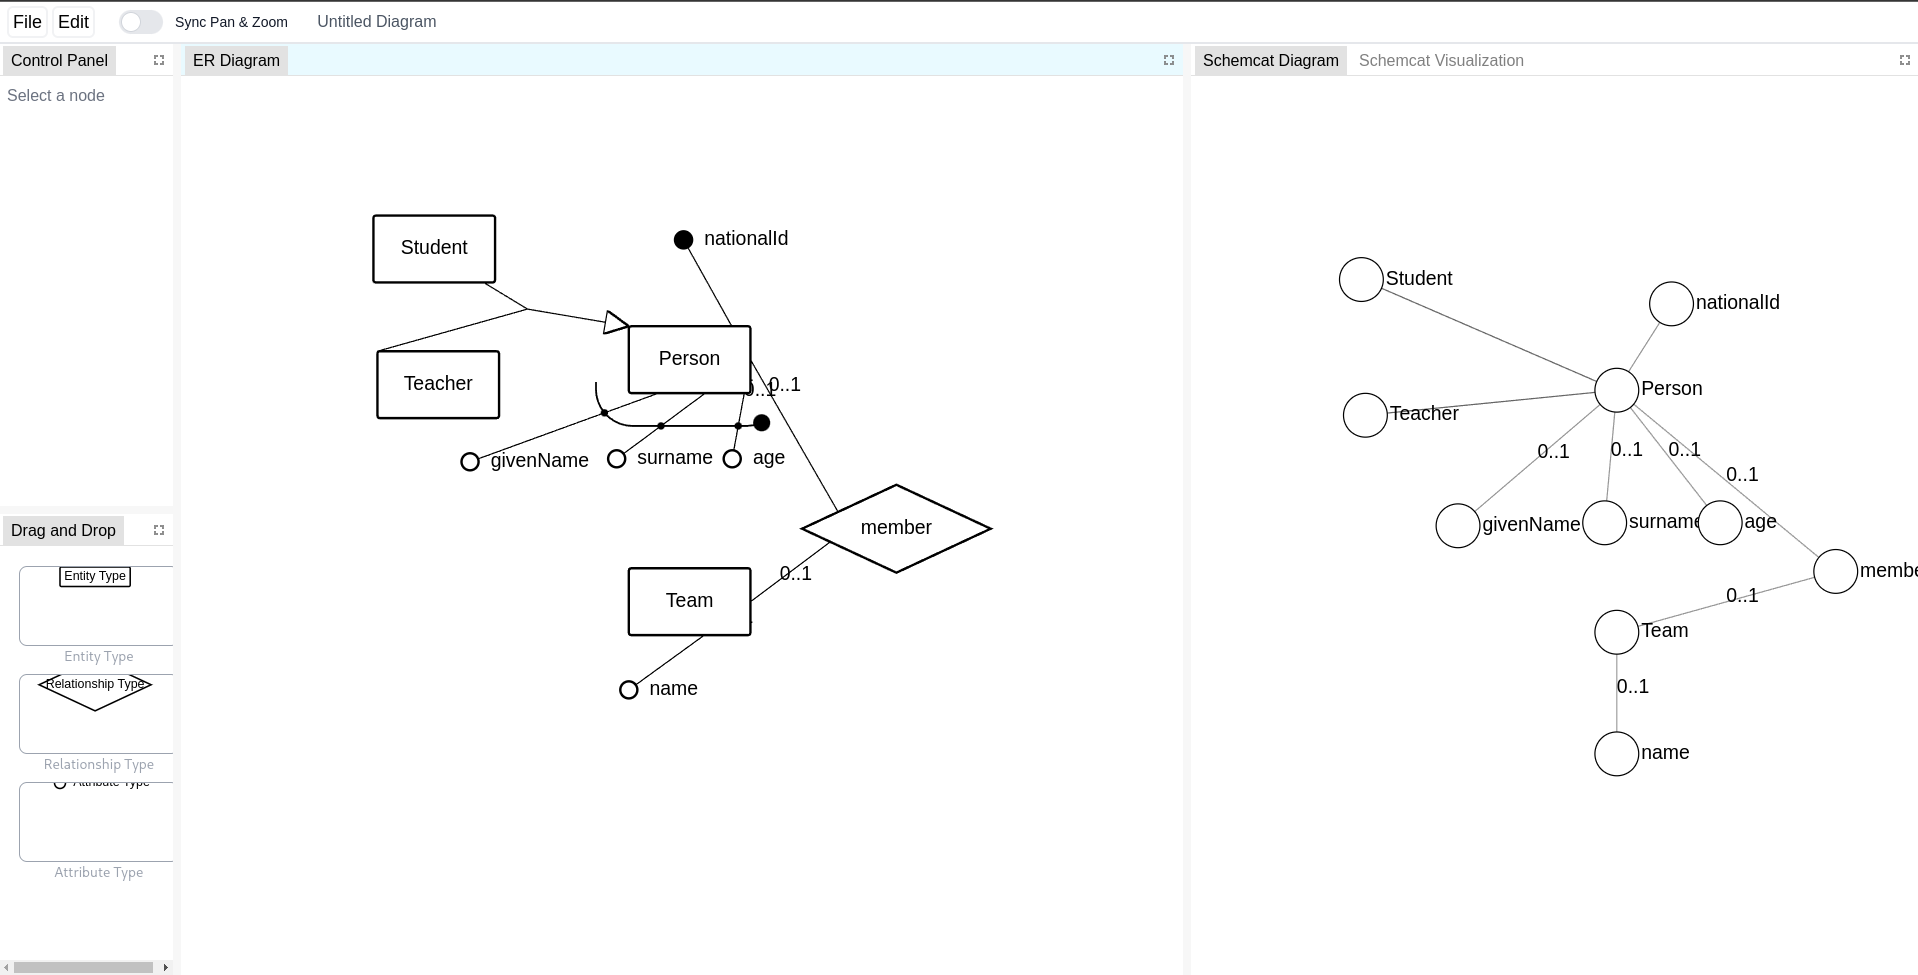
\includegraphics[width=\maxwidth{\textwidth}]{../img/app/user-interface.png}
  \caption{Ukázka uživatelského rozhraní aplikace}
  \label{fig:user-interface}
\end{figure}

V horní liště aplikace se nachází menu.
Tlačítko \menu{File} obsahuje možnosti pro vytvoření nového projektu a pro export.
Tlačítko \menu{Edit} obsahuje možnosti \menu{Undo} a \menu{Redo}.
Následuje přepínač \enquote{Sync Pan \& Zoom}, který zamkne synchronizaci pozice pláten.
Přetažení a přiblížení v jednom plátně tak způsobí totožný přesun a přiblížení ve všech ostatních plátnech.
Poslední položkou horní lišty je editovatelné textové pole s názvem diagramu.
Tento název se odráží v názvu souboru při exportu diagramu.

Rozhraní aplikace se skládá z oken, která obsahují záložky s různým obsahem.
Záložky lze přesouvat mezi okny a přetahovat přes jiné záložky myší, čímž může být vytvořeno nové okno.
Při přetahování je uživateli intuitivně vizuálně znázorněno, která z akcí se stane po puštění záložky myší.
Okna lze zvětšovat a zmenšovat přetažením jejich krajů.
Pokud v nějakém okně nezůstane ani jedna záložka, okno zanikne.

Právě aktivní okno je zvýrazněno světle modrou barvou.
Tato informace říká, kterým plátnem se bude řídit synchronizace pozic, a který diagram bude výchozí při exportování.

Záložka s názvem Control Panel obsahuje ovládací panel, ve kterém lze upravovat hodnoty jednotlivých vlastností elementů diagramu.
Lze ho pozorovat na Obrázku~\ref{fig:control-panel}, kde je zvoleno spojení, jehož kardinalitu a kotvy lze přenastavit v ovládacím panelu.

Záložka s popiskem Drag and Drop, která je také vidět na Obrázku~\ref{fig:control-panel} v levém dolním rohu, obsahuje konstrukty, které lze podržet a přesunout myší do plátna, čímž dojde k vytvoření daného konstruktu v daném plátně.

Význam záložek s popisky \acrshort{er} Diagram, Schemcat Diagram a Schemcat Visualization je zřejmý -- obsahují popořadě plátna pro \acrshort{er} diagram, schematickou kategorii a vizualizaci schematické kategorie.

\begin{figure}[!htb]
  \centering
  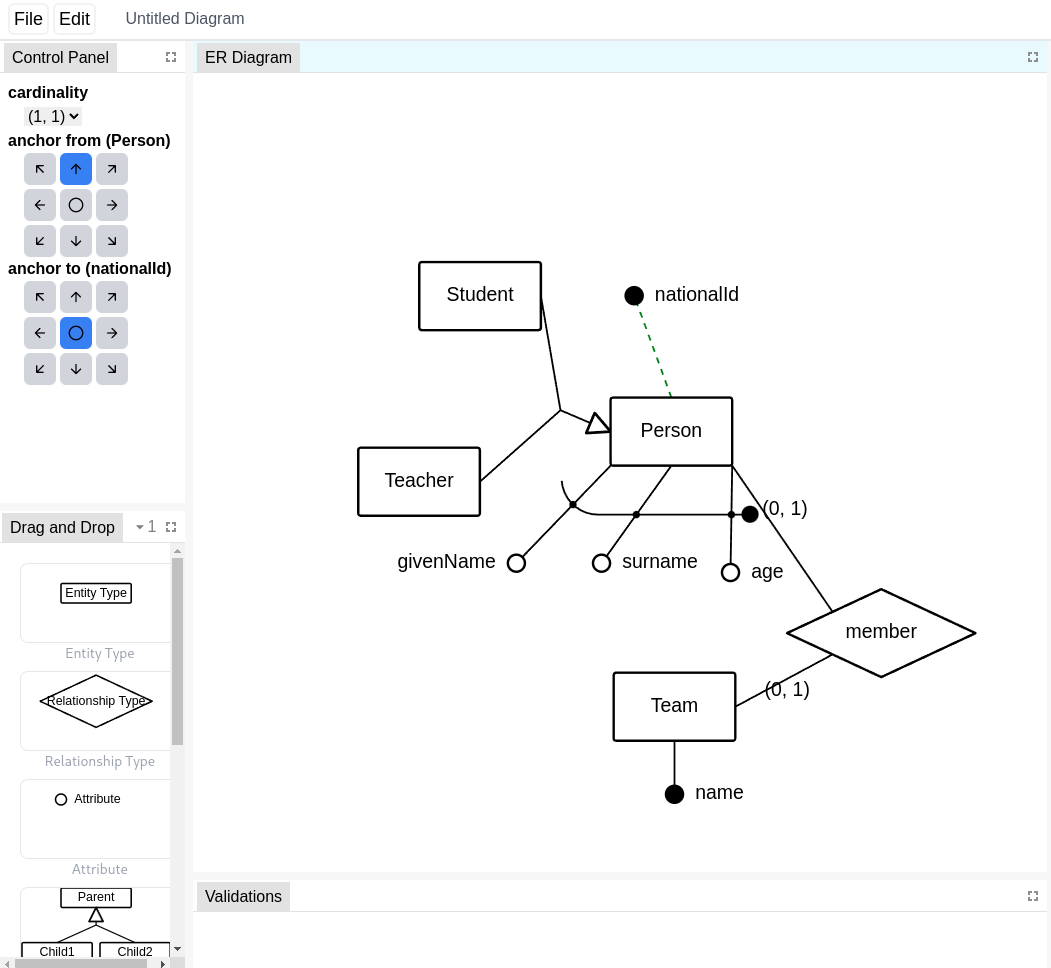
\includegraphics[width=\maxwidth{\textwidth}]{../img/app/control-panel.png}
  \caption{Ukázka ovládacího panelu}
  \label{fig:control-panel}
\end{figure}

\section{Technická dokumentace}

Zdrojový kód aplikace je k dispozici v elektronické příloze~\ref{appendix:electronic}.
Popíšeme zde některé důležité složky se zdrojovým kódem aplikace.

\begin{description}
  \item[\directory{src/components}] obsahuje React komponenty.
    Podsložky seskupují více podobných komponent.
    Některé z nich uvedeme.
  \item[\directory{src/components/UserControls}] seskupuje komponenty základních uživatelských prvků -- zaškrtávací pole, komponenta pro výběr barvy uživatelem, atd.
  \item[\directory{src/components/Menu}] seskupuje komponenty, které se týkají hlavního menu v horní liště aplikace a kontextového menu.
  \item[\directory{src/components/Dialog}] seskupuje komponenty dialogů pro export a potvrzování akcí.
  \item[\directory{src/hooks}] obsahuje React hooks, včetně důležitého \texttt{useStore.ts}, který obstarává instanci modelu s pomocí knihovny Zustand a jeho editaci pomocí knihovny Immer.
  \item[\directory{src/model}] obsahuje soubory, ve kterých se nacházejí jednotlivé třídy modelu.
  \item[\directory{src/utils}] obsahuje soubory s operacemi, které se týkají transformace textových řetězců, práce s poli, apod.
\end{description}

Vedle některých souborů, např.~\texttt{Array.ts}, jsou umístěny i soubory se stejným názvem, pouze odlišnou příponou, např.~\texttt{Array.test.ts}.
Tyto soubory obsahují unit testy, které ověřují funkcionalitu některých operací.

Vstupním bodem aplikace je soubor \directory{index.html}, který volá jediný skript -- \directory{src/main.tsx}.
Úkolem tohoto skriptu je do \acrshort{dom} stromu připojit framework React a vložit do něj hlavní komponentu aplikace.
Soubor obsahující hlavní komponentu aplikace je \directory{src/App.tsx}.
Tato komponenta se stará o přípravu uživatelského rozhraní za použití komponent z knihovny FlexLayout.
Do nich poté nasazuje vlastní komponenty aplikace.
Některé komponenty blíže popíšeme.

\begin{description}
  \item[ControlPanel] představuje ovládací panel, ve kterém uživatel mění hodnoty vlastností elementů diagramu.
    V modelu je pomocí dekorátorů (funkce jazyku TypeScript) určeno, který ovládací prvek má být použit pro kterou vlastnost třídy daného elementu.
    Tato informace je pak za běhu použita k použití správné komponenty.
    Jde o způsob reflexe, který je v TypeScriptu v době psaní práce experimentální (\texttt{reflect-metadata}).
  \item[AnchorPicker] slouží pro výběr kotvy, tj. bodu, kde má být přichyceno spojení na elementu diagramu.
  \item[Draggable] je obecná komponenta, která očekává děti a umožňuje jejich přetahování uživatelem.
  \item[ErNode] představuje element \acrshort{er} diagramu, tedy buď entitní typ, vztahový typ, nebo atribut.
    Který tvar vykreslí, rozhodne pomocí hodnoty typu \texttt{ErNodeType} z modelu.
  \item[IdentifierFence] je komponenta zodpovědná za vykreslování složených identifikátorů.
    Ty jsou vykresleny jako část obvodu obdélníku s oblými rohy, kterému říkáme \emph{fence} (neboli plot).
    V pracovní verzi se místo toho používaly Beziérovy křivky.
    Výsledek však nebyl dostatečně estetický.
  \item[PannableZoomableSvg] reprezentuje \acrshort{svg} plátno, které lze přesouvat, přibližovat a oddalovat myší.
    Dosahuje toho přepočítáváním \acrshort{svg} atributu \texttt{viewBox}.
\end{description}

Většina souborů obsahuje komentáře a TSDoc~\cite{microsoft_whattsdoc_} dokumentaci.

\section{Vývoj}\label{section:development}

K vývoji je potřeba mít nainstalovaný Node JS~\cite{openjsfoundation_nodejs_}.
Naše prostředí má Node verze 20.
Po instalaci by měl být k dispozici program \texttt{corepack}, kterým lze aktivovat náš upřednostňovaný správce balíčků \texttt{pnpm}~\cite{pnpm_pnpmfast_}.
Spustíme příkaz\footnote{rozsah \texttt{\^{}8} specifikuje verzi použitou v době psaní práce, nejnovější verzi lze nainstalovat tím, že místo tohoto rozsahu použijeme \texttt{latest}}
\begin{command}
corepack prepare --activate pnpm@^8
\end{command}
a poté ve složce \directory{schemcat} se zdrojovým kódem spustíme
\begin{command}
pnpm install
\end{command}
což nainstaluje všechny potřebné závislosti.

Poté lze používat všechny příkazy, které jsme definovali v souboru \texttt{package.json}.
Např.~příkaz
\begin{command}
pnpm run dev
\end{command}
spustí vývojový server, který sleduje změny ve zdrojovém kódu a sám stránku webového prohlížeče aktualizuje, když se kód změní.
To umožňuje rapidní cyklus vývoje a testování změn.

Příkaz
\begin{command}
pnpm run build
\end{command}
sestaví projekt a výsledné soubory připravené k nasazení uloží do složky \texttt{dist}.

\section{Instalace a nasazení}

Kromě zdrojového kódu je v Příloze~\ref{appendix:electronic} také sestavený projekt.
Stačí, aby správce soubory přesunul a nasadil na statický webový server.
Tento statický server však musí při odesílání souborů přes \acrshort{http} přiřazovat korektní \acrshort{mime} hlavičky, jinak není fungování projektu zaručeno.

Uživatel musí mít moderní webový prohlížeč, který podporuje ES6 moduly\footnote{prohlížeče definované v tabulce na této adrese \url{https://caniuse.com/es6-module}}.
Pokud je potřeba přidat podporu starších prohlížečů, je třeba postupovat podle Sekce~\ref{section:development}.
Dále nainstalovat balíček \texttt{@vitejs/plugin-legacy}\footnote{\url{https://www.npmjs.com/package/@vitejs/plugin-legacy}}.
Poté je třeba definovat v souboru \texttt{package.json} položku \texttt{browserslist} s rozsahem webových prohlížečů, které chceme podporovat podle specifikace\footnote{\url{https://browsersl.ist/}}.
Nakonec je nutné projekt sestavit.

Pokud chceme sestavený projekt spustit lokálně a máme nainstalovaný správce balíčků ze Sekce~\ref{section:development}, stačí spustit příkaz
\begin{command}
pnpx http-server .
\end{command}
ve složce se soubory sestaveného projektu.
Na obrazovce se pak vypíší lokální adresy, na kterých běží tento statický server.
